%!TEX root = OptimalOffline.tex
%input{Siddhartha}
\begin{theorem}
A transmission policy $\{\textbf{p},\textbf{s},N\}$ is an optimal solution to Problem 1 if and only if it satisfies the following structure.
\label{th_algo1_1}
\begin{align}
&\sum_{i=1}^{i=N}g(p_i)(s_{i+1}-s_i)=B_0; 								
\label{claim1}
\\
&\nonumber s_{N+1}-s_1=\mathcal{R}_0, 	 \ \ \ \ 						\text{ if } s_1>0 \text{ or }
\\
& s_{N+1}\le \mathcal{R}_0,				\ \ \ \ \ \ \ \ \ \				\text{ if } s_1=0;
\label{claim2}
\\
& \nonumber s_{n+1}=\argmin_{t_i: s_n < t_i \le s_{N+1}} \mathcal{P}(s_n,t_i)=\dfrac{\ETx(t_i^-)-U(s_n)}{t_i-s_n} \	\text{ and }
\\
&p_n=\mathcal{P}(s_{n},s_{n+1});\label{claim3}							
\\
&\exists s_j:s_j\in \textbf{s} \text{ and } s_j=Q.					
\label{claim4}
\end{align}
for $n=\{ 1,2,..,N\}$.
\end{theorem}
\begin{proof}
The proof consists of establishing both necessary and sufficiency conditions. First we work out the necessary part i.e. a optimal policy $\{\textbf{p},\textbf{s},N\}$ must have the given structure. We prove it by contradiction. We establish structure (\ref{claim3}) at first. Assume the optimal policy $\{\textbf{p},\textbf{s},N\}$ satisfies Lemmas 1-5 and does not satisfy structure (\ref{claim3}). Specifically, say the policy abides by the  structure (\ref{claim3}) from time $s_{1}$ to $s_n$, for some $n\in \{1,2,..,N\}$ but transmission power right after $s_n$ is not the minimum feasible constant power, i.e.
\begin{align}
p_n>\mathcal{P}(s_n,\tilde{s})\text{ where } \tilde{s}=\argmin_{t_i: s_n < t_i \le s_{N+1}} \mathcal{P}(t_i,s_n).\label{claim3_1}
\end{align}
Note that $p_n\nless \mathcal{P}(s_n,\tilde{s})$ as $\mathcal{P}(s_n,\tilde{s})$ is the minimum feasible power among all the epochs. The maximum energy that can used for transmission from time $s_{n}$ to $\tilde{s}$ is $\left(\ETx(\tilde{s}^-)-\ETx(s_{n}^-)\right)$, since the policy has used all the energy till time $s_{n}^-$, by Lemma \ref{lemma_energy_consumed}. If $\tilde{s}<s_{n+1}$, the transmission policy uses $p_n(\tilde{s}-s_{n})$ energy from time $s_n$ to $\tilde{s}$. If $\tilde{s}>s_{n+1}$, the transmission power during time $[s_{n+1},\tilde{s}]$ has to be greater than or equal to $p_n$ by Lemma \ref{lemma_increasing_power}. So the total energy used during period $[s_n,\tilde{s}]$ can be lower bounded by $p_n(\tilde{s}-s_{n})$. But, this energy is always more than the maximum energy available from $s_{n}$ to $\tilde{s}$ because
\begin{align}
&\nonumber\ETx(\tilde{s}^-)-\ETx(s_{n}^-)=\mathcal{P}(s_n,\tilde{s})(\tilde{s}-s_{n})<p_n(\tilde{s}-s_{n}),
\end{align}
where the inequality follows from (\ref{claim3_1}). This violates constraint (\ref{pb1_constraint_energy}) and contradicts the optimality of policy $\{\textbf{p},\textbf{s},N\}$.
 
Moving on to other structures, (\ref{claim1}) must be followed by the optimal policy as it is a constraint to the Problem 1 and (\ref{claim4}) follows from Lemma 5. We are left to prove structure (\ref{claim2}). $s_{N+1}-s_1\le \mathcal{R}_0$ by constraint (\ref{pb1_constraint_time}). If $s_1=0$ then we are done. When $s_1>0$, assume that $s_{N+1}-s_1<\mathcal{R}_0$. Now consider the policy where power vector is given by $\bm{\widetilde{p}}=\{p_1-\alpha,p_2,..,p_{N-1},p_N+\beta \}$ and the corresponding time vector be given by $\bm{\widetilde{s}}=\{s_1-\gamma,s_2,..,s_{N},s_{N+1}-\delta\}$, where $\gamma=\dfrac{\alpha}{p_1-\alpha}(s_2-s_1)$, $\delta =\dfrac{\beta}{p_N+\beta}(s_{N+1}-s_N)$ and $\alpha ,\beta$ are small positive constants. Since $(s_{N+1}-\delta)>s_{N+1}$, this policy finishes before the optimal policy $\{\textbf{p},\textbf{s},N\}$ and hence amounts to a contradiction only if we are able to show that it is feasible. By the definition of $s_i$ in (\ref{claim3}), $s_{2}$ is the first energy arrival which is on the boundary of energy constraint (\ref{pb1_constraint_energy}) i.e. $U(s_2)=\ETx(s_2^-)$ and $s_{N}$ is the last epoch satisfying $U(s_N)=\ETx(s_N^-)$. So we can choose arbitrarily small $\alpha ,\beta$ such that policy $\{\bm{\widetilde{p}},\bm{\widetilde{s}},N\}$ would be feasible with respect energy constraint (\ref{pb1_constraint_energy}). For every $\beta\rightarrow 0^+$ we can find a value of $\alpha$ such that the number of bits transmitted in policy $\{\bm{\widetilde{p}},\bm{\widetilde{s}},N\}$ remains the same as policy $\{\textbf{p},\textbf{s},N\}$ i.e. equal to $B_0$. So, excluding the common parts in the transmission policy $\{\textbf{p},\textbf{s},N\}$ and $\{\bm{\widetilde{p}},\bm{\widetilde{s}},N\}$, we can equate
\begin{align}
&g(p_N)(s_{N+1}-s_N)+g(p_1)(s_2-s_1)\nonumber
\\
&=g(p_1-\alpha)(s_2-s_1+\gamma)+g(p_N+\beta)(s_{N+1}-s_N-\delta)\nonumber,
\\
&\implies \delta(p_N+\beta)p_N\frac{1}{\beta}\left(\frac{g(p_N)}{p_N}-\frac{g(p_N+\beta)}{p_N+\beta}\right)\nonumber
\\
&=\gamma(p_1-\alpha)p_1\frac{1}{\alpha}\left(\frac{g(p_1-\alpha)}{p_1-\alpha}-\frac{g(p_1)}{p_1}\right).\label{bits_equal}
\end{align}
$\exists$ $p_N':p_N<p_N'<p_{N}+\beta$ and $p_1':p_1-\alpha<p_1'<p_{1}$ such that
\begin{align}
&\frac{d}{dp} \frac{g(p)}{p} \bigg{\vert}_{p=p_N'}=\frac{1}{\beta}\left(\frac{g(p_N+\beta)}{p_N+\beta}-\frac{g(p_N)}{p_N}\right),\label{diff_1}
\\
&\frac{d}{dp} \frac{g(p)}{p}\bigg{\vert}_{p=p_1'}=-\frac{1}{\alpha}\left(\frac{g(p_1-\alpha)}{p_1-\alpha}-\frac{g(p_1)}{p_1}\right)\label{diff_2}.
\end{align}
Substituting (\ref{diff_1}) and (\ref{diff_2}) into (\ref{bits_equal}) we get,
\begin{align}
&\delta(p_N+\beta)p_N\frac{d}{dp} \frac{g(p)}{p}  \bigg{\vert}_{p=p_N'}
=\gamma(p_1-\alpha)p_1\frac{d}{dp} \frac{g(p)}{p} \bigg{\vert}_{p=p_1'}.\label{bits_equal1}
\end{align}
It can be verified that $g(p)/p$ is decreasing function of $p$. As $p_1'<p_N'$, equation (\ref{bits_equal1}) implies $\gamma >\delta$. Hence the time for which transmission occurs in the policy $\{\bm{\widetilde{p}},\bm{\widetilde{s}},N\}$, $\left( s_{N+1}-s_1+\gamma-\delta\right)$, is greater than transmission time in policy $\{\textbf{p},\textbf{s},N\}$ i.e. $(s_{N+1}-s_1)$. As $s_{N+1}-s_1<\TRx_0$, we can choose arbitrarily small positive value of $\beta$ so that $(s_{N+1}-s_1)<(s_{N+1}-s_1+\gamma -\delta)<\TRx_0$ holds. So policy $\{\bm{\widetilde{p}},\bm{\widetilde{s}},N\}$ is feasible with constraints  (\ref{pb1_constraint_bits}), (\ref{pb1_constraint_energy}), (\ref{pb1_constraint_time}) and contradicts the optimality of policy $\{\textbf{p},\textbf{s},N\}$. This concludes that $s_{N+1}-s_1=\TRx_0$ (if $s_1\neq 0$) in optimal policy.

Next, we prove the sufficiency of the structure. Let the the policy $\{\textbf{p},\textbf{s},N\}$ follow  structure (\ref{claim1})-(\ref{claim4}). We need to show that this policy is optimal. Assume that there exists another policy given by $\{\textbf{p'},\textbf{s'},N'\}$ which abides by the Lemma 1-5 and is optimal, but does not follow the structure. We argue next that such a policy is not feasible and hence contradict its optimality. 

\textit{Case1}: If $s_1'>s_1\ge 0$, then by Lemma \ref{transmission_duration}, $s_{N'+1}'>s_{N+1}$. So policy $\{\textbf{p'},\textbf{s'},N'\}$ finishes after time $s_{N+1}$ and hence cannot be optimal. 

\textit{Case2}: Suppose $s_1'=s_1$. Let $s_i'$ be the first epoch for which $p_i'\ne p_i$ for some $i \in \{1,2,..,N\}$. By (\ref{claim3}), $p_i'>p_i$. 

If, in policy $\{\textbf{p'},\textbf{s'},N'\}$ transmission continues after $s_{i+1}$ i.e. $s_{N'+1}'>s_{i+1}$, then the amount of energy used by policy $\{ \textbf{p'},\textbf{s'},N'\}$ in interval $[s_{i},s_{i+1}]$ can be lower bounded by $p_i'(s_{i+1}-s_i)$, by Lemma \ref{lemma_increasing_power}. $p_i'(s_{i+1}-s_i)$ is more than $p_i(s_{i+1}-s_i)$, which is the energy used by policy $\{\textbf{p},\textbf{s},N\}$. But by Lemma \ref{lemma_energy_consumed}, $\{\textbf{p},\textbf{s},N\}$ uses all energy available by $s_{i+1}$. So policy $\{\textbf{p'},\textbf{s'},N'\}$ is not feasible with respect to the energy constraint. 

If $s_{N'+1}'\le s_{i+1}$, then it can be easily verified by (\ref{property_decreasing}) that policy $\{\textbf{p'},\textbf{s'},N'\}$ transmits strictly less number of bits in interval $[s_i,s_{N'+1}]$ than the other policy in interval $[s_{i},s_{i+1}]$. Both policies being same till $s_i$, we conclude that policy $\{\textbf{p'},\textbf{s'},N'\}$ transmits less than $B_0$  bits and thus it is not optimal.

\textit{Case3}: This case argues the infeasibility when $s_1'<s_1$. Unlike other cases this case is more laborious. The idea of the proof is to show that if a policy starts its transmission early and finishes earlier than policy $\{\textbf{p},\textbf{s},N\}$, it always takes more transmission time, which is going to violate the time constraint (\ref{pb1_constraint_time}). First, we establish that the policy $\{\textbf{p'},\textbf{s'},N'\}$ must be same as policy $\{\textbf{p},\textbf{s},N\}$ from epoch $s_2$ to an epoch $s_j$ such that $s_j=\displaystyle\max_{s_i<s_{N'+1}'} s_i$. Let $s_k'=\displaystyle\max_{s_i'<s_2}s_i'$ and transmission continues with constant power $p_k'$ till $s_{k+1}'$. Clearly $s_{k+1}\ge s_2$. If $s_{k+1}'>s_2$, then transmission with a constant power $\dfrac{\ETx(s_1'^-)}{(s_{k+1}'-s_1)} $ from $s_1$ to $s_{k+1}'$ is feasible and $\dfrac{\ETx(s_{k+1}'^-)}{(s_{k+1}'-s_1)}<\dfrac{\ETx(s_2^-)}{(s_2-s_1)}=p_1$. This contradicts ($\ref{claim3}$). So, $s_{k+1}'=s_2$. Now, let $p_{k+1}'\neq p_2$ and $s_j>s_3$. From definition of $p_2$, $p_{k+1}>p_2$. Then the amount of energy used by policy $\{\textbf{p'},\textbf{s'},N'\}$ between $s_2$ and $s_3$ is more than what is harvested. So $p_{k+1}'=p_2$ ($s'_{k+2}=s_3$) and similarly, we can show that $p'_{k+2}=p_3$.. ($ s'_{k+3}=s_4$..) till epoch $s_j$. By Lemma 5 and (\ref{claim4}) we can be sure that there exists atleast one epoch $s_i$ which belongs to $\textbf{s}$ as well as $\textbf{s'}$ i.e. $j\ge 2$.

\begin{figure}[htb]
\centering
\centerline{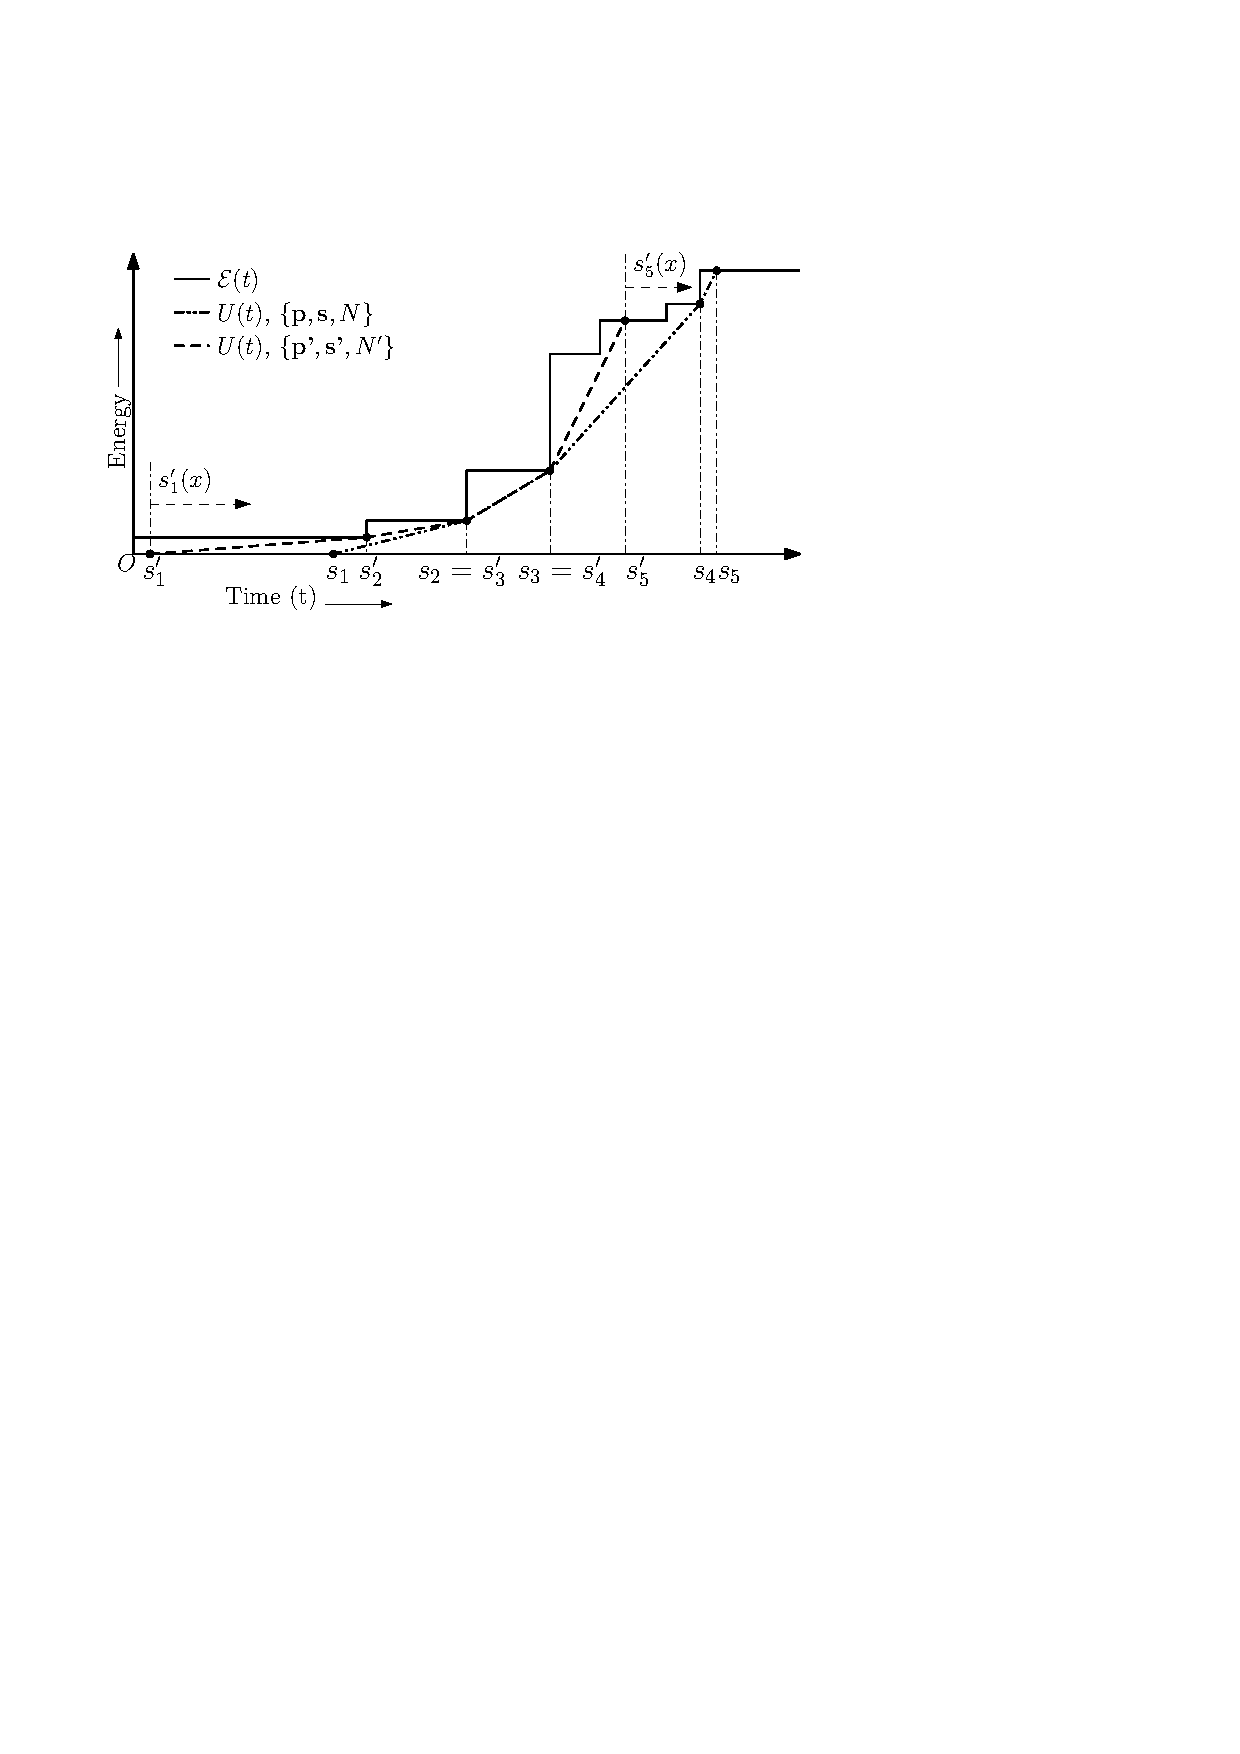
\includegraphics[width=8cm]{Theorem1_sufficient.pdf}}
\caption{Energy curves at Transmitter explaining \textit{Case3} in proof of Theorem \ref{th_algo1_1}}
\label{Theorem1_figure}
\end{figure}

Now, consider the following process which creates child feasible policies from policy $\{\textbf{p'},\textbf{s'},N'\}$ as shown in Figure \ref{Theorem1_figure}. We define two pivots $pv_1$ and $pv_2$. Initially we set $pv_1=s_2'$ and $pv_2=s_{N'}'$. The transmission power right before $pv_1$ is $u$ ($u=p_1'$ initially) and right after $pv_2$ is $v$ ($v=p_{N'}'$ initially). Keeping the policy same from $pv_1$ to $pv_2$ we increase $u$ by a small amount to $u+du$ and decrease $v$ by a small amount to $v-dv$ such that the number of bits transmitted ( i.e. $B_0$) remains same under this transformation. Let $s_1'$ change to $s_1'+x$ and $s_{N'+1}'$ change to $s_{N'+1}'+y$ for some $x,y>0$. We denote such a policy by vectors $\{\textbf{p'(x)},\textbf{s'(x)},N'(x)\}$. Following the argument provided while proving the necessary statement of this Theorem, we can conclude that $(s_{N'(x)+1}'(x)-s_1'(x))<(s_{N'+1}'-s_1')$. We continue increasing $x$ till either $u=p_2$ (in which case we change $pv_1=s_2$) or $v=p_{N'-1}'$ (where we change $pv_2=s_{N'-1}'$) or $s_{N'(x)+1}'(x)$ hits an epoch, say $t_j$ ($pv_2=t_j$, $v\rightarrow\infty$ in this case). After this, we again start increasing $x$ with changed definitions. We continue this process till $x=s_1-s_1'$  or $u$ becomes equal to $v$. Note that the former stopping criteria will be met at a smaller $x$ than the later one since policy $\{\textbf{p'(x)},\textbf{s'(x)},N'(x)\}$ shares at least one epoch with policy $\{\textbf{p},\textbf{s},N\}$ by arguments of previous paragraph. By maintaining these rules we ensure that policy $\{\textbf{p'(x)},\textbf{s'(x)},N'(x)\}$ abides by Lemma 1-5 and is feasible with energy constraint. Since $\left( s_{N'(x)+1}'(x)-s_1'(x)\right)$ is decreasing with $x$, the policy is also feasible with time constraint. As this is continuous on $x$, at $x=s_1-s_1'$ we reach a policy such that $s_1'(x)=s_1$. For $x=s_1-s_1'$, if $s_{N'(x)+1}'(x)\ge s_{N+1}$ then $s_{N'+1}'-s_1'>s_{N'(x)+1}'(x)-s_1'(x)\ge \TRx_0$ and policy $\{\textbf{p'},\textbf{s'},N'\}$ is infeasible with time constraint. If $s_{N'(x)+1}'(x)< s_{N+1}$ then we can follow the arguments in \textit{Case2} to show that policy $\{\textbf{p'(x)},\textbf{s'(x)},N'(x)\}$ is infeasible, which in turn accounts for the infeasibility of policy $\{\textbf{p'},\textbf{s'},N'\}$.
\end{proof}

























%input{Rushil}
\begin{theorem}
The transmission policy, which results from the algorithm presented in Table \ref{Algorithm1}, is an optimal solution to Problem 1.
\label{th_algo1_2}
\end{theorem}


\begin{proof}
To prove that the policy (say $\{\textbf{p},\textbf{s},N\}$) described by Algorithm \ref{Algorithm1} is optimal, it is sufficient to show that it abides by the structure presented in Theorem \ref{th_algo1_1}.

To begin with, we prove that the power allocations in Algorithm \ref{Algorithm1} are increasing. We prove this by induction. The base case constitutes of showing that, the initial feasible solution has increasing powers. If we begin with the constant power policy from time $R$ to $S$ with power $p_c=\frac{\ETx(t_n)}{S-R}=\frac{\ETx(t_n)-\ETx(Q^-)}{S-Q}$, then we are done. 

Suppose we solve for Algorithm 1 from \cite{Yang} with $B_2$ bits to transmit after time $Q$, then the transmission power after time $Q$ is always increasing. Now, we need to prove that transmission power $p_c$ between time $S$ and $Q$ is less than the transmission power just after time $Q$(say $p_i$). Let transmission with $p_i$ end at epoch $t_i$. We prove it by contradiction. Assume that $p_i<p_c$. Following two cases arise.

\textit{Case1:} If $t_i<S$, energy consumed by $p_c$ between time $Q$ to $t_i$ is 
\begin{align}
&p_c(t_i-Q)>p_i(t_i-Q)=(\ETx(t_i^-)-\ETx(Q^-))\label{eq_1_algo1_modified}
\end{align}
Since $p_c$ uses all energy by $Q$, the maximum amount of energy available for transmission between $Q$ and $t_i$ is $(\ETx(t_i^-)-\ETx(Q^-))$. But by \eqref{eq_1_algo1_modified}, $p_c$ is infeasible between time $Q$ and $t_i$. As transmitting with $p_c$ was always feasible between $Q$ and $S$ (and therefore between $Q$ and $t_i$) in constant power policy, we reach a contradiction.        

\textit{Case2:} If $t_i>S$, then $\ETx(t_i^-)>\ETx(S)=\ETx(t_n)$. So, 
\begin{align}
g(p_i)(t_i-Q)&=g\left(\frac{\ETx(t_i^-)-\ETx(Q^-)}{t_i-Q}\right)(t_i-Q)
\\
&>g\left(\frac{\ETx(t_n)-\ETx(Q^-)}{t_i-Q}\right)(t_i-Q)
\\
&>g\left(\frac{\ETx(t_n)-\ETx(Q^-)}{S-Q}\right)(S-Q)\label{eq_2_algo1_modified}
\\
&=g(p_c)(S-Q)=B_2.
\end{align}
where \eqref{eq_2_algo1_modified} follows from Property P4. So transmission with $p_i$ from $Q$ to $t_i$ departs more than $B_2$ bits. This is inconsistent with the assumption that the solution we get from Algorithm 1 in \cite{Yang} exactly transmits $B_2$ bits after $Q$. 

Having proved the base case, assume that transmission powers from Algorithm \ref{Algorithm1} are increasing in its $n^{th}$ iteration. In $(n+1)^{th}$ iteration,   
 
First we prove that the power allocations in Algorithm \ref{Algorithm1} are in accordance with \eqref{claim3}. In any particular iteration of the algorithm, we select the maximum transmission power between $t_{l}$ and all epochs before lying in range $t_{start}$ to $t_l$. Let $t_j$ be the epoch which amounts to the maximum power and $p_j$ be the maximum power, i.e. 
\begin{align}
&t_j=\argmax_{t_i:t_{start}\le t_i< t_l} \max\left(\frac{\ETx(t_l^-)-\ETx(t_i^-)}{t_l-t_i}, \frac{\ETx(t_l^-)}{t_l-t_{start}}\right)
\\
&p_j= \max_{t_i:t_{start}\le t_i< t_l} \max\left(\frac{\ETx(t_l^-)-\ETx(t_i^-)}{t_l-t_i}, \frac{\ETx(t_l^-)}{t_l-t_{start}}\right)
\label{eq_max_algo1_2}
\end{align}
We claim that this is indeed the maximum over all $t_i$'s in range $s_1$ to $t_l$. To prove this by contradiction, assume that $\exists t_{a}: s_1\le t_{a}<t_{start}$ and $p_{a}=\dfrac{\ETx(t_l^-)-\ETx(t_a^-)}{t_l-t_a}>p_j $. From \eqref{eq_max_algo1_2}, we can say that 
\begin{align}
&\ETx(t_l^-)\le p_j(t_l-t_{start}),\\
&\implies \ETx(t_l^-)<p_a(t_l-t_{start}).
\end{align}
But transmission with power $p_a$ consumes $p_a(t_l-t_{start})$ amount of energy between $t_j$ and $t_l$, which is more than the maximum available energy till $t_l$ i.e. $\ETx(t_l^-)$. Hence transmission with $p_a$ is infeasible. 

 
Now we seek to show that this procedure of selecting maximum slopes going 'backwards' also gives us the minimum slopes going 'forwards', as described in \eqref{claim3}.\\
We shall show this by contradiction. Let $t_i$, $t_j$ and $t_k$ be three consecutive corner points where the power of transmission increases, as per our allocation. Now suppose, it is possible to transmit with a lower power between $t_i$ and some $t'_j$. 
Then the power of transmission between $t_j$ and $t_k$ is not the maximum power since we could transmit at a higher power from $t'_j$ and $t_k$. Which is a contradiction as this is not consistent with out allocation algorithm.\\
Therefore, the allocation policy before point $Q$ is consistent with the structure.. (See figure)
We can prove similarly for the powers after point $Q$.
\end{proof}




